\section{Scenario introduction}\label{sc:scenarioIntroduction}
% Scenario introduction
A marathon runner is racing a track shaped as shown in figure \ref{fig:scenarioIntroduction}, while equipped with sensor node A. It broadcasts four packets per second tracking the runner’s heart rate. The level of details in the tracking package defines the number of marathons possible for the runner to run before a new battery is required. At one time the track was closed, resulting in the runner racing around the building of her workplace.
%TODO: Forstår ikke de sidste to linjer i den.

\begin{figure}[H]
	\centering
	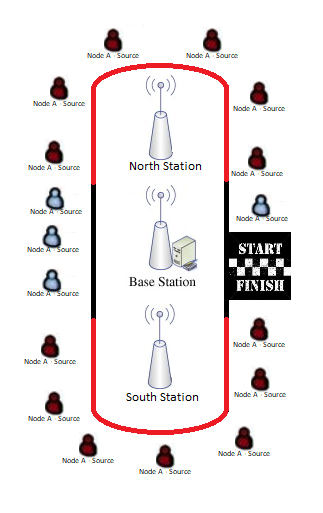
\includegraphics[width=\linewidth]{introduction/scenario/fig/scenarioIntroduction.png}
	\caption{A marathon runner "node A" is racing around a track, while transmitting pulse information to the base station. In the red northern territory, node A transmits to the north station which relays the message to the base station. Likewise, at the southern station.}
	\label{fig:scenarioIntroduction}
\end{figure}

\section{Protocol introduction “To hop or not to hop”}\label{sc:protocolIntroduction}
The base station will be requesting data from the runner node with a packet size of 128 bytes and save it in storage. When the base station is out of range, the north or the south relay station will receive the request and relay it to the runner. Time Synchronization, Localization and Scalability will be considered regarding the protocol design. Each and combined scenarios will be evaluated in relation to signal strength relative to power consumption and data reliability.
%TODO: Det gør vi vel ikke? Tænker at skrive: We will look at energy costs and signal strentch when deciding to hop or not.